\def\year{2017}\relax
\documentclass[letterpaper]{article}
\usepackage{aaai17}
\usepackage{times}
\usepackage{helvet}
\usepackage{courier}

% Packages added by Rob
% Also: grffile, latexsym, textcomp, longtable, booktabs, amsmath, amsfonts, amssymb?
\usepackage{amsmath}
\usepackage[utf8]{inputenc}
\usepackage{url}
\usepackage{graphicx}
\providecommand{\tightlist}{\setlength{\itemsep}{0pt}\setlength{\parskip}{0pt}}%

% Packages added by Josh
\usepackage{amsmath}

\frenchspacing
\setlength{\pdfpagewidth}{8.5in}
\setlength{\pdfpageheight}{11in}
\pdfinfo{
/Title (Insert Your Title Here)
/Author (Put All Your Authors Here, Separated by Commas)}
\setcounter{secnumdepth}{0}
\begin{document}

\title{ConceptNet 5.5: An Open Multilingual Graph of General Knowledge}
\author{Author list withheld for blind review}

\maketitle


\section{Abstract}\label{abstract}

Machine learning about language can be improved by supplying it with specific knowledge and sources of external information. We present here a new version of the linked open data resource ConceptNet that is particularly well suited to be used with modern NLP techniques such as word embeddings.

ConceptNet is a knowledge graph that connects words and phrases of natural language with labeled edges. Its knowledge is collected from many sources that include expert-created resources, crowd-sourcing, and games with a purpose. It is designed to represent the general knowledge involved in understanding language, improving natural language applications by allowing the application to better understand the meanings behind the words people use.

When ConceptNet is combined with word embeddings acquired from distributional semantics (such as word2vec), it provides applications with understanding that they would not acquire from distributional semantics alone, nor from narrower resources such as WordNet or DBPedia. We demonstrate this with state-of-the-art results on intrinsic evaluations of word relatedness that translate into improvements on applications of word vectors, including solving SAT-style analogies.


\section{Introduction}\label{introduction}

ConceptNet is a knowledge graph that connects words and phrases of
natural language (\emph{terms}) with labeled, weighted edges
(\emph{assertions}). The original release of ConceptNet \cite{liu2004conceptnet}
was intended as a parsed representation of Open Mind Common Sense
\cite{singh2002omcs}, a crowd-sourced knowledge project. This paper
describes the release of ConceptNet 5.5, which has expanded to include
lexical and world knowledge from many different sources in many
languages.

ConceptNet represents relations between words such as:

\begin{itemize}
    \item A \emph{net} is used for \emph{catching fish}.
    \item ``\emph{Leaves}'' is a form of the word ``\emph{leaf}''.
    \item The word \emph{cold} in English is \emph{studený} in Czech.
        % TODO: this might not be good Portuguese
    \item O \emph{alimento} é usado para \emph{comer} [Food is used for eating].
\end{itemize}

In this paper, we will concisely assertions such as the above as triples of
their start node, relation label, and end node: the assertion that ``a dog has
a tail'' can be represented as (\emph{dog}, \emph{HasA}, \emph{tail}).

ConceptNet also represents links between knowledge resources. In addition to
its own knowledge about the English term \emph{astronomy}, for example,
ConceptNet contains links to URLs that define \emph{astronomy} in WordNet,
Wiktionary, UMBEL, and DBPedia.

The graph-structured knowledge in ConceptNet can be particularly useful to NLP
learning algorithms, particularly those based on word embeddings, such as
\cite{mikolov2013word2vec}. We can use ConceptNet to build semantic spaces that
are more effective than distributional semantics alone.

The most effective semantic space is one that learns from both distributional
semantics and ConceptNet, using a generalization of the ``retrofitting'' method
\cite{faruqui2015retrofitting}. We call this hybrid semantic space ``ConceptNet
Numberbatch'', to clarify that it is a separate artifact from ConceptNet
itself.

ConceptNet Numberbatch performs significantly better than other systems across
many evaluations of word relatedness, and this increase in performance
translates to improvements on downstream tasks such as analogies.  On Turney's
corpus of SAT-style analogy questions \cite{turney2005lra}, its accuracy of
56.4\% is slightly higher than the previous best system (Turney's LRA) and only
slightly lower than the performance of the average human test-taker.

Building word embeddings is not the only application of ConceptNet, but it is a
way to apply ConceptNet that achieves clear benefits and is compatible with
ongoing research in distributional semantics. This shows the continued relevance of
ConceptNet, and of explicitly collecting knowledge to improve the computational
understanding of semantics.

In this paper, we will begin by describing ConceptNet 5.5 and its features,
show how to use ConceptNet alone as a semantic space and a measure of word
relatedness, and then proceed to describe and evaluate the hybrid system
ConceptNet Numberbatch on these various semantic tasks.

\section{Structure of ConceptNet}\label{structure-of-conceptnet}

\subsection{Knowledge Sources}\label{knowledge-sources}

ConceptNet 5.5 is built from the following sources:

\begin{itemize}
\item
  Facts acquired from Open Mind Common Sense (OMCS) \cite{singh2002omcs}
  and sister projects in other languages \cite{anacleto2006portuguese}
  \cite{eckhardt2008kid}
\item
  Information extracted from parsing Wiktionary, in multiple languages,
  with a custom parser (``Wikiparsec'')
\item
  ``Games with a purpose'' designed to collect common knowledge
  \cite{vonahn2006verbosity} \cite{nakahara2011nadya} \cite{kuo2009petgame}
\item
  Open Multilingual WordNet \cite{bond2013linking}, a linked-data
  representation of WordNet \cite{miller1998wordnet} and its parallel
  projects in multiple languages
\item
  JMDict \cite{breen2004jmdict}, a Japanese-multilingual dictionary
\item
  OpenCyc \cite{matuszek2006cyc}, a hierarchy of hypernyms provided by
  Cyc, a system that represents common sense knowledge in predicate
  logic
\item
  A subset of DBPedia \cite{auer2007dbpedia}, a network of facts
  extracted from Wikipedia infoboxes
\end{itemize}

With the combination of these sources, ConceptNet contains over 21
million edges and over 8 million nodes. Its English vocabulary contains
approximately 1,500,000 nodes, and there are 83 languages in which it
contains at least 10,000 nodes.

The largest source of input for ConceptNet is Wiktionary, which provides
18.1 million edges and is mostly responsible for its large multilingual
vocabulary. However, much of the character of ConceptNet comes from OMCS
and the various games with a purpose, which express many different kinds
of relations between terms, such as \emph{PartOf} (``a wheel is part of
a car'') and \emph{UsedFor} (``a car is used for driving'').


\subsection{Relations}\label{relations}

ConceptNet uses a closed class of selected relations such as \emph{IsA},
\emph{UsedFor}, and \emph{CapableOf}, intended to
represent a relationship independently of the language or the source of
the terms it connects.

ConceptNet 5.5 aims to align its knowledge resources on its core set of 36
relations. These generalized relations are similar in purpose to WordNet's
relations such as \emph{hyponym} and \emph{meronym}, as well as to the qualia
of the Generative Lexicon theory \cite{pustejovsky1991generative}.

Relations with specific semantics, such as \emph{UsedFor} and
\emph{HasPrerequisite}, tend to connect common words and phrases, while
rarer words are connected by more general relations such as
\emph{Synonym} and \emph{RelatedTo}.

ConceptNet's edges are directed, but as a new feature in ConceptNet 5.5,
some relations are designated as being symmetric: \emph{SimilarTo},
\emph{RelatedTo}, \emph{EtymologicallyRelatedTo}, \emph{Synonym},
\emph{Antonym}, and \emph{DistinctFrom}. The directionality of these
edges is unimportant. The assertion (\emph{A}, \emph{SimilarTo},
\emph{B}) is considered equivalent to (\emph{B}, \emph{SimilarTo},
\emph{A}).


\subsection{Term Representation}\label{term-representation}

ConceptNet represents terms in a standardized form. The text is
Unicode-normalized (in NFKC form) and lowercased, and split into
non-punctuation tokens using the tokenizer in the Python package
\texttt{wordfreq} \cite{speer2016wordfreq}, which builds on the standard Unicode word
segmentation algorithm. The tokens are joined with underscores, and this
text is prepended with the URI \texttt{/c/lang}, where \emph{lang} is
the BCP 47 language code for the language the term is in. As an example,
the English term ``United States'' becomes
\texttt{/c/en/united\_states}. Relations have a separate namespace of
URIs prefixed with \texttt{/r}, such as \texttt{/r/PartOf}.

Previous versions of ConceptNet required terms in English to be in lemmatized
form, so that, for example, ``United States'' had to be represented as
\texttt{/c/en/unite\_state}. In this representation, ``drive'' and ``driving'' were
the same term, allowing the assertions (\emph{car}, \emph{UsedFor},
\emph{driving}) and (\emph{drive}, \emph{HasPrerequisite}, \emph{have license})
to be connected. ConceptNet 5.5 removes the lemmatizer, and instead
relates inflections of words using the \emph{FormOf} relation. The two
assertions above are now linked by the third assertion (\emph{driving},
\emph{FormOf}, \emph{drive}), and both ``driving'' and ``drive'' can be looked
up in ConceptNet.


\subsection{Vocabulary}\label{vocabulary}

When building a knowledge graph, the decision of what a node should
represent has significant effects on how the graph is used. It also has
implications that can make linking and importing other resources
non-trivial, because different resources make different decisions about
their representation.

In ConceptNet, a node is a word or phrase of a natural language, often a
common word in its undisambiguated form. The word ``lead'' in English is
a term in ConceptNet, represented by the URI \texttt{/c/en/lead}, even
though it has multiple meanings. The advantage of ambiguous terms is
that they can be extracted easily from natural language, which is also
ambiguous. This representation is equivalent to that used by systems
that learn distributional semantics from text, such as word2vec
\cite{mikolov2013word2vec}.

ConceptNet's representation allows for more specific, disambiguated
versions of a term. The URI \texttt{/c/en/lead/n} refers to noun senses
of the word ``lead'', and is effectively included within
\texttt{/c/en/lead} when searching or traversing ConceptNet, and
linked to it with the implicit relation \emph{SenseOf}. Many data
sources provide information about parts of speech, allowing us to use
this as a common representation that provides a small amount of
disambiguation. Further disambiguation is allowed by the URI structure,
but not currently used.

\subsection{Linked Data}

ConceptNet imports knowledge from some other systems, such as WordNet, into its
own representation. These other systems have their own target vocabularies that
need to be aligned with ConceptNet, which is usually an underspecified,
many-to-many alignment.

A term that is imported from another knowledge graph will be connected to
ConceptNet nodes via the pseudo-relation \emph{ExternalURL}, pointing to an
absolute URL that represents that term in that external resource.  This
preserves the provenance of the data and enables looking up what the
untransformed data was.

As ConceptNet terms can also be given absolute URLs
(by prefixing their local URI with the domain name
\url{http://api.conceptnet.io}), this allows ConceptNet to participate in the
broader ecosystem of Linked Open Data.

\section{Related Work}

ConceptNet is the knowledge graph version of the Open Mind
Common Sense project \cite{singh2002omcs}, a large common sense knowledge base
of the most basic things a person knows.

Many projects strive to create lexical resources of general knowledge.  Cyc
\cite{matuszek2006cyc} has built an ontology of common-sense knowledge in
predicate logic form over the decades. DBPedia \cite{auer2007dbpedia} extracts
knowledge from Wikipedia infoboxes, providing a large number of facts, largely
focused on named entities that have Wikipedia articles. The Google Knowledge
Graph \cite{singhal2012googleblog} is perhaps the largest and most general
knowledge graph, though its content is not freely available. It focuses largely
on named entities that can be disambiguated, with a motto of ``things, not
strings''.

ConceptNet's role compared to these other resources is to provide a
sufficiently large, free knowledge graph that focuses on the meanings of words
(not named entities) as they are used in natural language. This focus on words
makes it particularly compatible with the idea of representing word meanings as
vectors.

Word embeddings represent words as dense unit vectors of real numbers, where
vectors that are close together are semantically related. This representation
is appealing because it represents meaning as a continuous space, where
similarity and relatedness can be treated as a metric. Word embeddings are
often produced as a side-effect of a machine learning task, such as predicting
a word in a sentence from its neighbors.  This approach to machine learning
about semantics is sometimes referred to as \emph{distributional semantics} or
\emph{distributed word representations}, and it contrasts with the
knowledge-driven approach of semantic networks or knowledge graphs.

Two prominent matrices of embeddings are the word2vec embeddings trained on 100
billion words of Google News using skip-grams with negative sampling
\cite{mikolov2013word2vec}, and the GloVe 1.2 embeddings trained on 840 billion
words of the Common Crawl \cite{pennington2014glove}. These matrices are
downloadable, and we will be using them both as a point of comparison and as
inputs to an ensemble. \citeauthor{levy2015embeddings}
\shortcite{levy2015embeddings} evaluated multiple embedding techniques and the
effects of various explicit and implicit hyperparameters, produced their own
performant word embeddings using a truncated SVD of words and their contexts,
and provided recommendations for the engineering of word embeddings.

Holographic embeddings \cite{nickel2015holographic} are embeddings learned from
a labeled knowledge graph, under the constraint that a circular correlation of
these embeddings gives a vector representing a relation. This representation
seems extremely relevant to ConceptNet. In our attempt to implement it on
ConceptNet so far, it has converged too slowly to experiment with, but this
could be overcome eventually with some optimization and additional computing
power.

\section{Applying ConceptNet to Word Embeddings}

\subsection{Computing ConceptNet Embeddings Using PPMI}

We can represent the ConceptNet graph as a sparse, symmetric term-term matrix.
Each cell contains the sum of the weights of all edges that connect the two
corresponding terms. For performance reasons, when building this matrix, we
prune the fringe of the ConceptNet graph, discarding terms connected to fewer
than three edges.

We consider this graph to represent terms and their contexts. In a corpus of
text, the context of a term would be the terms that appear nearby in the text;
here, the context is the other nodes it is connected to in ConceptNet. From
this representation, we can calculate word embeddings directly from the
ConceptNet graph by following the practical recommendations of
\citeauthor{levy2015embeddings} \shortcite{levy2015embeddings}.

As in Levy et al., we determine the pointwise mutual information of the matrix
entries with context distributional smoothing, clip the negative values to
yield positive pointwise mutual information (PPMI), reduce the dimensionality
of the result to 300 dimensions with truncated SVD, and combine the terms and contexts
symmetrically into a single matrix of word embeddings.

This gives a matrix of word embeddings we call ConceptNet-PPMI.  These
embeddings implicitly represent the overall graph structure of ConceptNet, and
allow us to compute the approximate connectedness of any pair of nodes.

We can expand ConceptNet-PPMI to restore the nodes that we pruned away,
assigning them vectors that are the average of their neighboring nodes.

\subsection{Combining ConceptNet with Distributional Word Embeddings}

Having created embeddings from ConceptNet alone, we would now like to create
a more robust set of embeddings that represents both ConceptNet and distributional
word embeddings learned from text.

Retrofitting \cite{faruqui2015retrofitting} is a process that adjusts an
existing matrix of word embeddings using a knowledge graph. Retrofitting
infers new vectors $q_i$ with the objective of being close to their original
values, $\hat{q_i}$, and also close to their neighbors in the graph with edges $E$,
by minimizing this objective function:
$$\Psi(Q) = \sum_{i=1}^{n}\left[
    \alpha_i \lVert q_i - \hat{q_i} \rVert ^2 + \sum_{(i, j) \in E} \beta_{ij} \lVert q_i - q_j \rVert ^2
\right] $$

\citeauthor{faruqui2015retrofitting} give a simple iterative process to minimize
this function over the vocabulary of the original embeddings.

The process of ``expanded retrofitting'', first described in
\cite{speer2016ensemble}, can optimize this objective over a larger vocabulary,
including terms from the knowledge graph that do not appear in the vocabulary
of the word embeddings. This effectively sets $\alpha_i = 0$ for terms whose
original values are undefined. We set $\beta_{ij}$ according to the weights
of the edges in ConceptNet.

The particular benefit of expanded retrofitting to ConceptNet is that it can
benefit from the multilingual connections in ConceptNet. It learns more about
English words via their translations in other languages, and gives these
foreign-language terms embeddings in the same space as the English terms.

We add one more step to retrofitting, which is to subtract the mean of the
vectors that result from retrofitting, then re-normalize them to unit vectors.
Retrofitting has a tendency to move all vectors closer to the vectors for
highly-connected terms such as ``person''. Subtracting the mean helps to ensure
that terms remain distinguishable from each other.

\subsection{Combining Multiple Sources of Embeddings}

Retrofitting can be applied to any existing matrix of word embeddings, without
needing access to the data that was used to train them. This is particularly
useful because it allows building on publicly-released matrices of embeddings
whose input data is unavailable or difficult to acquire.

As described in the ``Related Work'' section, word2vec and GloVe both provide
recommended pre-trained matrices. These matrices represent somewhat different
domains of text and have complementary strengths, and the way that we can
benefit from them the most is by taking both of them as input.

To do this, we apply retrofitting to both matrices, then find a globally
linear projection that aligns the results on their common vocabulary.
This process was inspired by \citeauthor{zhao2015learning} \shortcite{zhao2015learning}.
We find the projection by concatenating the columns of the matrices and reducing
them to 300 dimensions using truncated SVD. We then use this alignment to infer
compatible embeddings for terms that are missing from one of the vocabularies.

In ongoing work, we are experimenting with additionally including
distributional word embeddings from corpora of non-English text in this merger.
Preliminary results show that this improves the multilingual performance of the
embeddings.

After retrofitting and merging, we have a labeled matrix of word embeddings
whose vocabulary is derived from word2vec, GloVe, and the pruned ConceptNet
graph. As in ConceptNet-PPMI, we re-introduce all the nodes from ConceptNet by
looking up and averaging their neighboring nodes.

\section{Evaluation}

To compare the performance of fully-built systems of word embeddings, we will
first compare their results on intrinsic evaluations of word relatedness, then
apply the word embeddings to the downstream tasks of solving proportional
analogies and choosing the sensible ending to a story, to evaluate whether
better embeddings translate to better performance on semantic tasks.

The hybrid system described above is the system we name ConceptNet Numberbatch,
with the version number 16.09 indicating that it was built in September 2016.
We now compare results from ConceptNet Numberbatch 16.09 to other systems:
word2vec SGNS trained on Google News \cite{mikolov2013word2vec}, GloVe 1.2
trained on the Common Crawl \cite{pennington2014glove}, and a recently-released
system that was not used in ConceptNet Numberbatch: LexVec, whose embeddings
are trained on the English Wikipedia and NewsCrawl \cite{salle2016lexvec}.
Additionally, we compare to the ConceptNet-PPMI embeddings, showing what performance
can be achieved with ConceptNet and no other data.

\subsection{Evaluations of Word Relatedness}
\label{intrinsic-evaluations}

One way to evaluate the intrinsic performance of a semantic space is to ask it
to rank the relatedness of pairs of words, and compare its judgments to human
judgments.\footnote{It is sometimes important to distinguish \emph{similarity}
from \emph{relatedness}. For example, the term ``coffee'' is related to
``mug'', but coffee is not \emph{similar} to a mug. What a machine can learn
from the connectivity of ConceptNet is focused on relatedness.} If one word in
a pair is out-of-vocabulary, the pair is assumed to have a relatedness of 0. A
good semantic space will provide a ranking of relatedness that is highly
correlated with the human gold-standard ranking, as measured by its Spearman
correlation ($\rho$).

Many gold standards of word relatedness are in common use. Here, we focus on
MEN-3000 \cite{bruni2014men}, a large crowd-sourced ranking of common words; RW
\cite{luong2013rw}, a ranking of rare words; WordSim-353 \cite{finkelstein2001ws},
a smaller evaluation that has been used as a benchmark for many methods; and MTurk-771
\cite{halawi2012mturk}, another crowd-sourced evaluation of a variety of words.
To avoid manually overfitting by designing our semantic space around a
particular evaluation, we experimented using smaller development sets, holding
out some test data until it was time to include results in this paper:

\begin{itemize}
\item
    MEN-3000 is already divided into a 2000-item development set and a
    1000-item test set. We use the results from the test set as the final results.
\item
    RW has no standard dev/test breakdown. We sampled 2/3 of its items as
    a development set and held out the other 1/3 (every third line of the file,
    starting with the third).
\item
    We used all of WordSim-353 in development.
\item
    We did not use MTurk-771 in development, holding out the entire set
    as a final test, showing that ConceptNet Numberbatch performs well on a
    previously-unseen evaluation.
\end{itemize}

\subsection{Solving SAT-style Analogies}

Proportional analogies are statements of the form ``$a_1$ is to $b_1$ as $a_2$
is to $b_2$''. The task of filling in missing values of a proportional analogy
was common until recently on standardized tests such as the SAT. Now, it is
popular as a way to show that a semantic space can approximate relationships
between words, even without taking explicit relationships into account.

Much of the groundwork for evaluating systems' ability to solve proportional
analogies was laid by Peter Turney, including his method of Latent Relational
Analysis \cite{turney2005lra}, which was quite effective at solving
proportional analogies by repeatedly searching the Web for the words involved
in them. A newer method called SuperSim \cite{turney2013supersim} does
not require Web searching. These methods are evaluated on a dataset of 374 SAT
questions that Turney and his collaborators have collected. Unfortunately, the
questions are not licensed for free distribution, but Turney provides them on
request.

Many of the best results on this evaluation have been achieved by Turney in his
own work. One interesting system not by Turney is BagPack
\cite{herdagdelen2009bagpack}, which could learn about analogies either from
unstructured text or from ConceptNet 4.

Solving analogies over word embeddings is often described as comparing the
difference $b_2 - a_2$ to $b_1 - a_1$ \cite{mikolov2013word2vec}, but for the
task of filling in the best pair for $a_2$ and $b_2$, it helps to take
advantage of more of the structure of the question to provide more constraint
than this single comparison.

In a sensible analogy, the words on the right side of the analogy will be
related in some way to the words on the left side, so we should aim for some
amount of relatedness between $a_1$ and $a_2$, and between $b_1$ and $b_2$,
regardless of what the other terms are. Also, in many cases, a satisfying
analogy will still make sense when it is transposed to ``$a_1$ is to $a_2$ as
$b_1$ is to $b_2$''. The analogy ``fire : hot :: ice : cold'', for example, can
be transposed to ``fire : ice :: hot : cold''.

This gives us three components that we can weigh to evaluate whether a pair
($a_2$, $b_2$) completes an analogy: their separate similarity to $a_1$ and
$b_1$, the dot product of differences between the pairs, and the dot product of
differences between the transposed pairs.  The total weight does not matter, so
we can put these together into a vector equation with two free parameters:
\begin{equation*}
    \begin{split}
        s &= a_1 \cdot a_2 + b_1 \cdot b_2\\
          &  + w_1(b_2 - a_2) \cdot (b_1 - a_1)
             + w_2(b_2 - b_1) \cdot (a_2 - a_1)
    \end{split}
\end{equation*}

The appropriate values of $w_1$ and $w_2$ depend on the nature of the
relationships in the analogy questions, and also on how these relationships
appear in the vector space. We optimize these parameters separately for each
system we test, using grid search over a number of possible values so that each
system can achieve its best performance. The grid search is performed on
odd-numbered questions, holding out the even-numbered questions for a final
evaluation.

The weights found for ConceptNet Numberbatch were $w_1 = 0.35$ and $w_2 =
0.65$, with other word embeddings choosing similar values. This indicates,
surprisingly, that the transposed form of the analogy was often more important
than the directly stated form of the analogy for choosing the best answer pair.

\subsection{An Evaluation of Common-Sense Stories}
\label{story-evaluation}

The Story Cloze Test \cite{mostafazadeh2016cloze} is a recent evaluation of
semantic understanding that tests whether a method can choose the sensible
ending to a simple story. Prompts consist of four sentences that tell a story,
and two choices are provided for a fifth sentence that concludes the story,
only one of which makes sense.

This task is distinguished by being very challenging for computers but very
easy for humans, because of the extent that it relies on implicit, common sense
knowledge. Most systems that have been evaluated on the Story Cloze Test
score only marginally above the random baseline of 50\%, while a typical
human agrees with the gold standard answers 100\% of the time.

Our preliminary attempt to apply ConceptNet Numberbatch to the Story Cloze Test
is to use a very simple ``bag-of-vectors'' model, by averaging the
embeddings of the words in the sentence and choosing the ending whose average is
closest. This allows us to compare directly to one of the original results presented by
\citeauthor{mostafazadeh2016cloze}, in which a bag of vectors using GenSim's
implementation of word2vec scores 53.9\% on the test set.

This bag-of-vectors model uses no knowledge of how one event might sensibly
follow from another, only which words are related in context. Improving the
score of this model should not be portrayed as actual ``story understanding'',
but it recognizes that sensible stories do not suddenly change topic.

\section{Results and Discussion}
\begin{figure}[t]
\centering
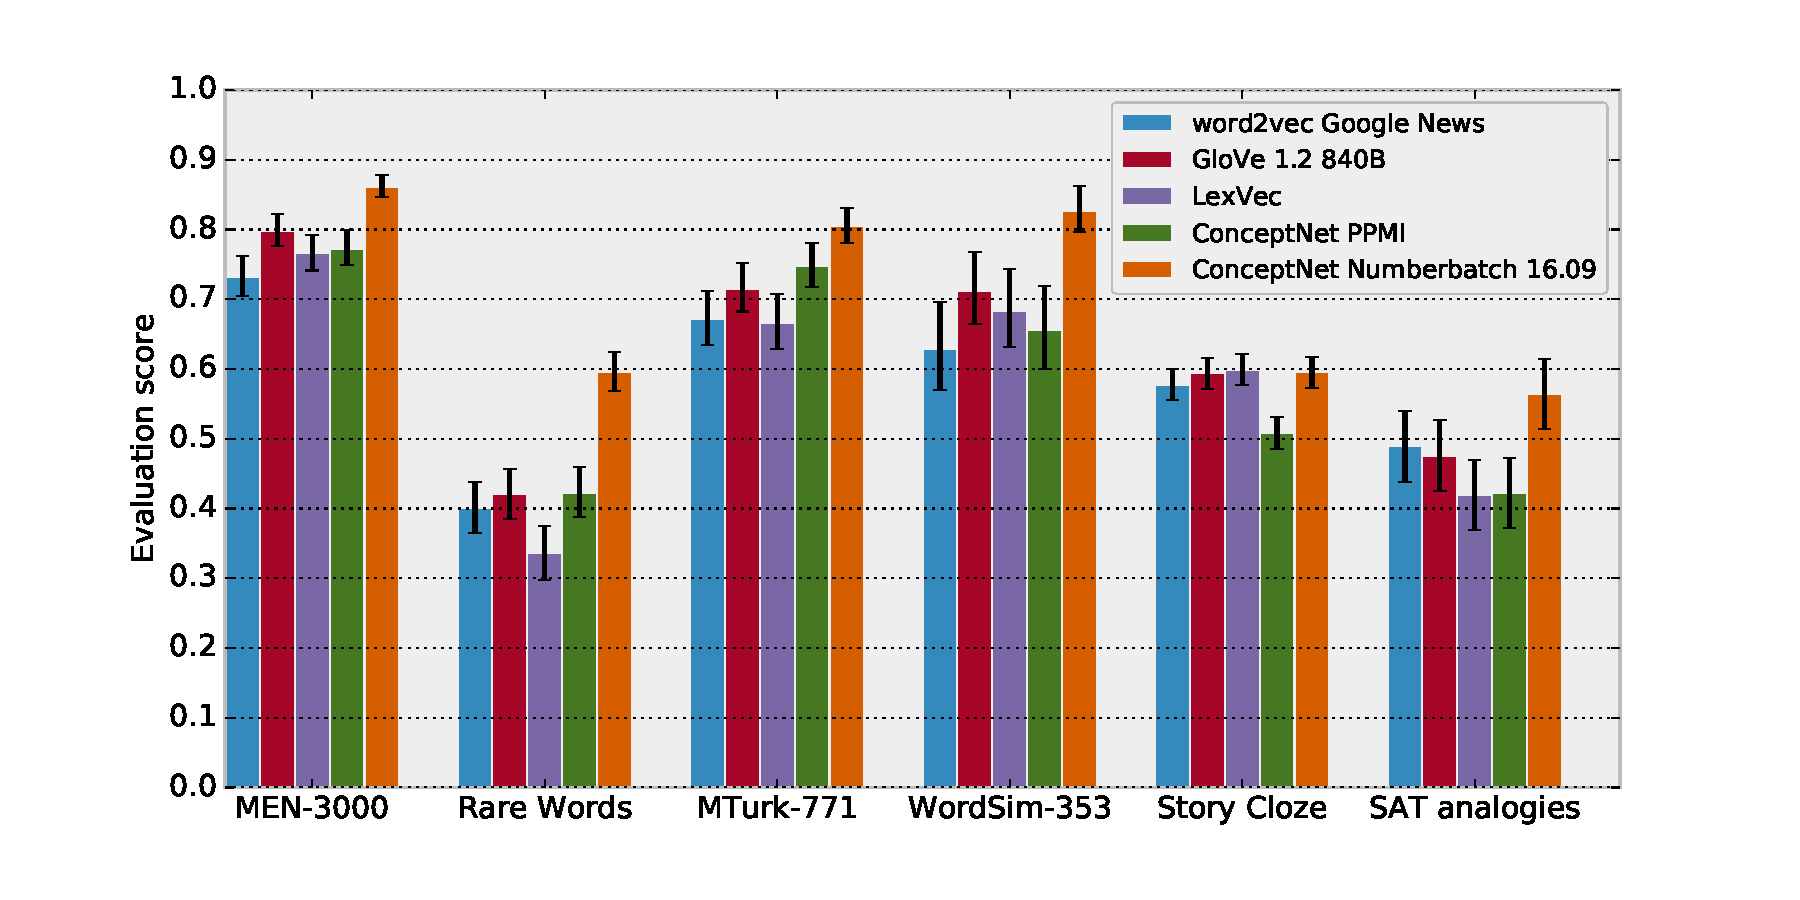
\includegraphics[width=3.3in]{eval-graph.pdf}
\caption{
    Performance of word embeddings across multiple evaluations.
    Error bars show 95\% confidence intervals.
}
\label{eval-results}
\end{figure}

\begin{table}[t]
\centering
\begin{tabular}{lrrr}
\bf Evaluation     & \bf Dev & \bf Test & \bf Final \\
\hline
MEN-3000 ($\rho$)              & .853 & .861 & .861 \\
Rare Words ($\rho$)            & .603 & .578 & .596 \\
MTurk-771 ($\rho$)             &  --- & .804 & .804 \\
WordSim-353 ($\rho$)           & .827 &  --- & .827 \\
Story Cloze Test (acc)         & .604 & .595 & .595 \\
SAT Analogies (acc)            & .545 & .583 & .564
\end{tabular}
\caption{The Spearman correlation ($\rho$) or accuracy (acc) of ConceptNet Numberbatch 16.09, our hybrid system,
on data used in development and data held out for testing.}
\label{eval-table}
\end{table}

Figure~\ref{eval-results} compares the performance of the systems we compared
across all evaluations. For word-relatedness evaluations, the Y-axis represents
the Spearman correlation ($\rho$), using the Fisher transformation to compute a
95\% confidence interval that assumes the given word pairs are sampled from an
unobservable larger set \cite{bonett2000sample}. For the analogy and story evaluations,
the Y-axis is simply the proportion of questions answered correctly, with 95\%
confidence intervals calculated using the binomial exact test.

The scores of our system on all these evaluations appear in
Table~\ref{eval-table}, including a development/test breakdown that shows no
noticeable overfitting. The ``Final'' column is meant for comparisons to other
papers and used in the graph. It uses the standard test set if it exists (which
is the case for MEN-3000 and Story Cloze), or all of the data
otherwise.

On the four word-relatedness evaluations, ConceptNet Numberbatch 16.09 (the
complete system described in this paper) is state of the art, performing
significantly better than all other systems evaluated. Its high scores on both
the Rare Words dataset and the crowd-sourced MEN-3000 and MTurk-771 datasets
shows both the breadth and the depth of its understanding of words.

ConceptNet Numberbatch also performed the best at SAT analogies, getting 56.4\%
of the questions correct (58.3\% on the half that was held out for final
testing), with a 95\% confidence interval of 51.4\%--61.4\%.
This compares to LRA \cite{turney2005lra}, which scored 56.1\% and was
allowed to search AltaVista during the evaluation, as well as the previous best
self-contained system, SuperSim \cite{turney2013supersim}, which scored 54.8\%.
This also compares to the performance of the average human college applicant,
said by Turney and Littman to be 57.0\%.

The analogy results show that our word embeddings have a level of understanding
of words that has traditionally been sought in college applicants. This is the
case even though the system, like many others, is only adding and subtracting
values that measure the relatedness of terms; it uses no particular
representation of what the relationships between these terms actually are.

It seems likely that there exists a way to take ConceptNet's relation labels
into account and do even better at analogies. We have not yet found such a
method that performs better than a simple comparison of word relatedness, and
in ongoing research, we are continuing to look for one. But for now, we have
shown that knowledge-informed word embeddings are up to the challenge of SAT
analogies, and do not need to be relegated to a synthetic analogy data set
designed only for testing word embeddings.

The performance of our system on the Story Cloze Test was acceptable but
unremarkable.  ConceptNet Numberbatch chose the correct ending 59.5\% of the
time, which is in fact slightly better than any results reported by
\citeauthor{mostafazadeh2016cloze} \shortcite{mostafazadeh2016cloze}, including
neural nets trained on the task. However, we could also achieve a similar score
by using the same bag-of-vectors approach on other word embeddings. The best
score of 59.9\% was achieved by LexVec, with Numberbatch, GloVe, and word2vec
all within its margin of error.

This result should perhaps be comforting to those who aim to improve the
computational understanding of stories.  A ``bag of vectors'' approach  may be
marginally more successful at choosing the correct ending to a story than other
approaches, but the performance of this approach has likely reached a plateau.
It seems that any sufficiently high-quality word embeddings can choose the
correct ending about 59\% of the time, based on nothing but the assumption that
the end of a story should be similar to the rest of it. This should perhaps be
taken as a baseline: any representation designed to usefully represent the
events in stories should get more than 59\% correct.

We have compared word embeddings that represent only distributional semantics
(word2vec, GloVe, and LexVec), word embeddings that represent only relational
knowledge (ConceptNet PPMI), and the combination of the two (ConceptNet
Numberbatch), and we have shown that the whole is more than the sum of its
parts.

ConceptNet continues to be important in a field that has come to focus on word
embeddings, because word embeddings can benefit from what ConceptNet knows.
ConceptNet can make word embeddings more robust and more human-like, as shown
by the state-of-the-art results that ConceptNet Numberbatch achieves at
matching human judgments on multiple evaluations.

Any technique built on word embeddings should
consider including a source of relational knowledge, or starting from a
pre-trained set of word embeddings that has taken relational knowledge into
account. One of the many goals of ConceptNet is to provide this knowledge in a
convenient form that can be applied across many domains and many languages.

\section{Availability of This Code and Data}

% TODO: make Zenodo citations for Numberbatch

The code for building and evaluating ConceptNet and its embeddings is part of
the ConceptNet 5 codebase, developed at \url{http://github.com/commonsense/conceptnet5}.
The output embeddings, ConceptNet Numberbatch 16.09, are archived on the research
repository Zenodo at [FIXME].

\section{Acknowledgments}

We would like to thank the tens of thousands of volunteers who provided the
crowd-sourced knowledge that makes ConceptNet possible. This includes
contributors to Open Mind Common Sense and its related projects, as well as
contributors to Wikipedia and Wiktionary, who are improving the state of
knowledge for humans and computers alike.

\bibliographystyle{aaai}
\bibliography{conceptnet-paper}

\end{document}
